\chapter{Detector Applications to measuring the active brain}

\section{{F}unctional {N}ear-{I}nfrared {fNIR} Imaging}
% detector applicaitons to improving fNIR
\begin{figure}[b]
  \begin{center}
    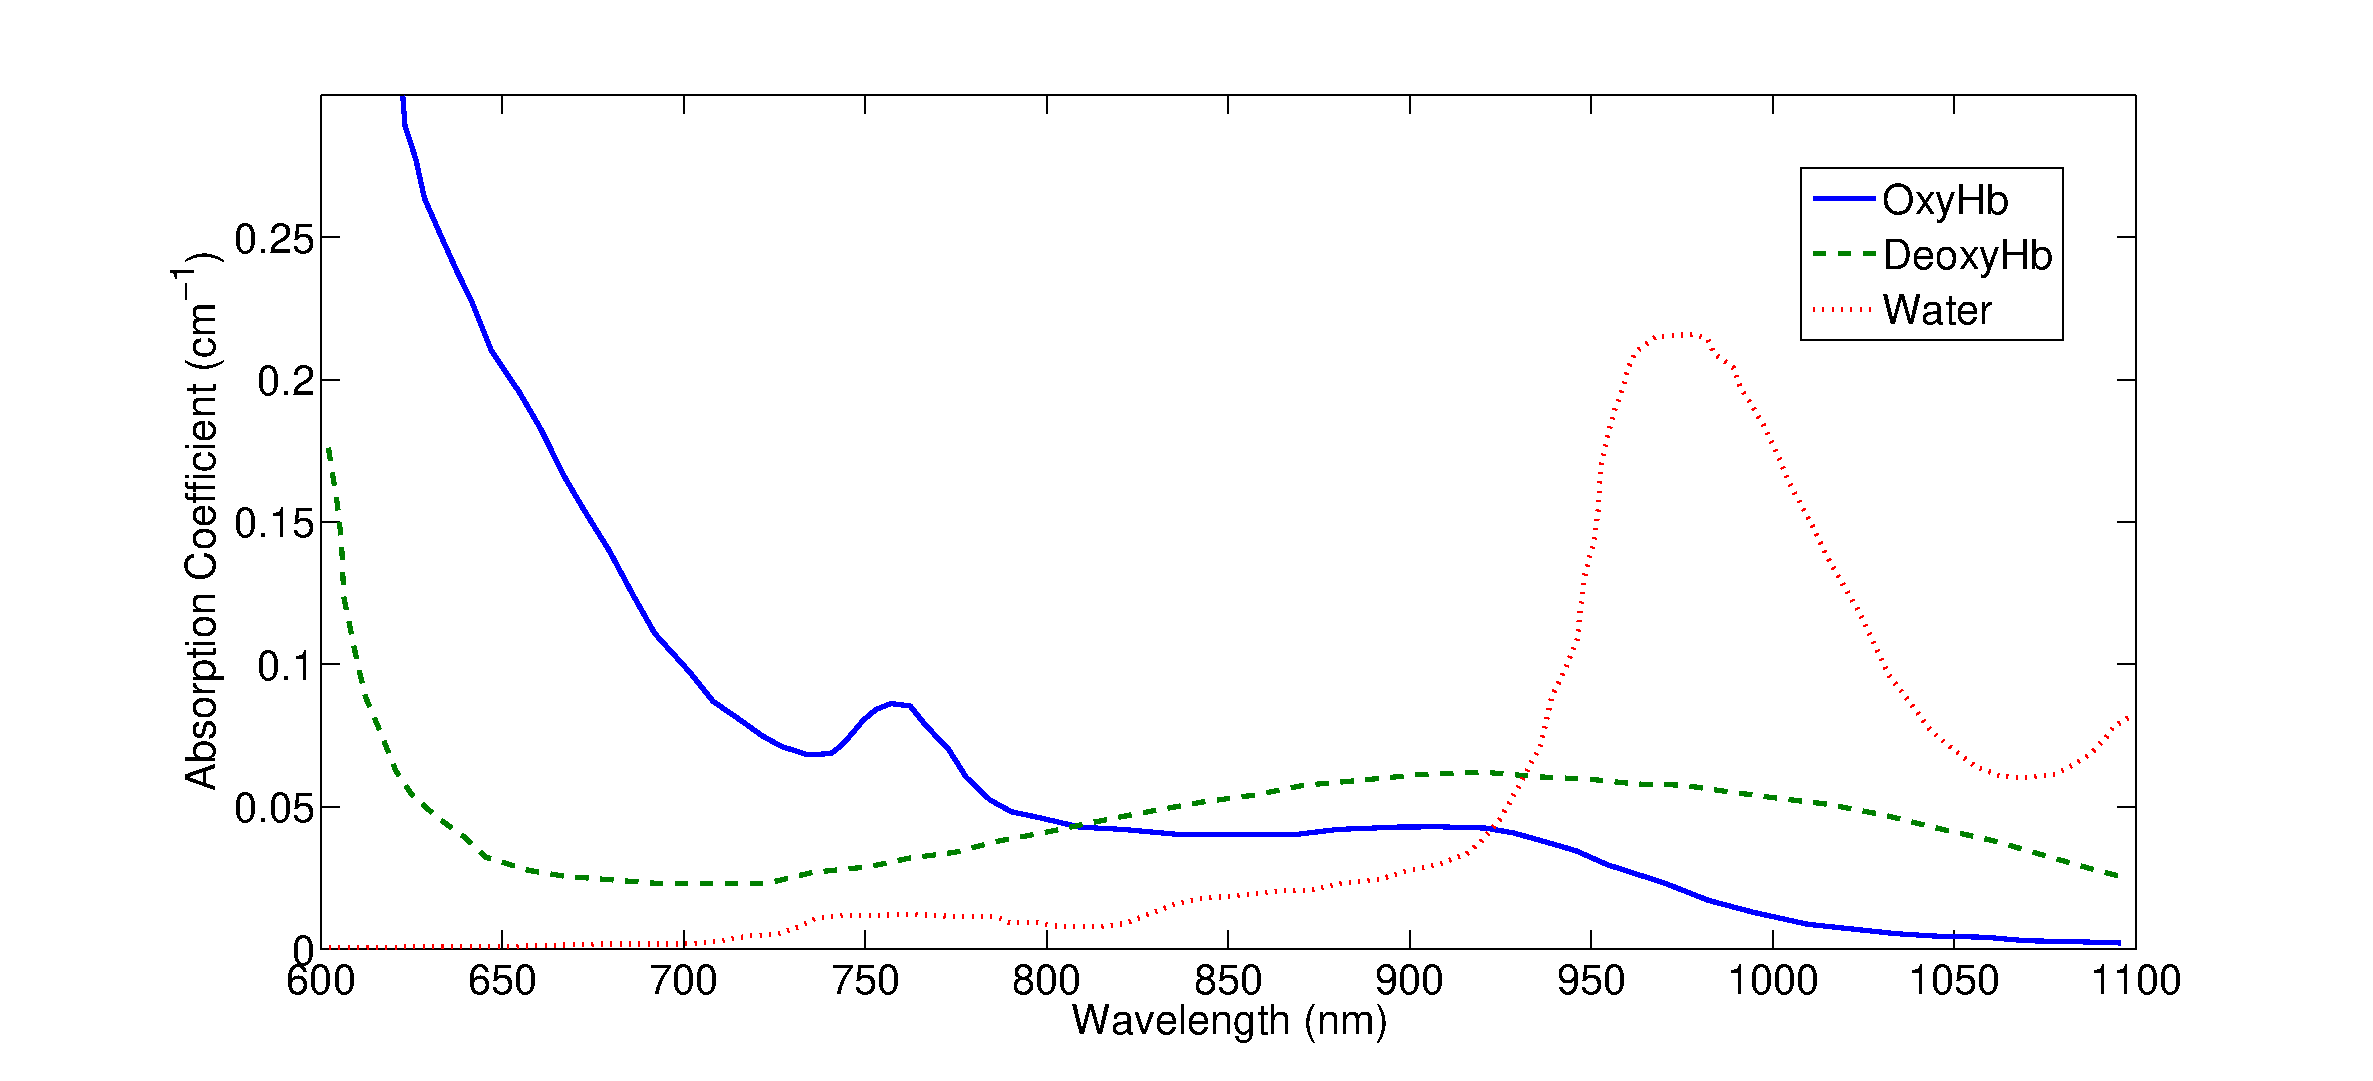
\includegraphics{AbsorptionData}
    \caption[Absorption spectra of water, deoxyhemoglobin and oxyhemoblogin]{\label{fig:fnirabsorption} Absorption spectra of water, Hb and Dhb.  From \citet{cope} and HB stuff from \citet{horecker} }
  \end{center}
\end{figure}

As discussed in previous sections, changes in tissue activity can be detected by measuring the change in blood oxygenation levels.  Functional Magnetic Resonance Imaging (fMRI) is one technique for accomplishing this (through measuring the BOLD response), but other techniques exist.  

The blood oxygenation can be determined by measuring the relative concentrations of oxyhemoglobin (oxy-Hb) and deoxyhemoglobin (deoxy-Hb).  Since oxy-Hb and deoxy-Hb have different absorption spectra (\cref{fig:fnirabsorption}), it is possible to determine this through optical techniques.

\begin{align}
  \label{eq:o2bloodvolume}
  Oxygenation\ &= \Delta C_{HBO2} - \Delta C_{HB} \nonumber \\
  Blood\ Volume\ &= \Delta C_{HBO2} + \Delta C_{HB} 
\end{align}

\begin{equation}
  I = I_0 e^{-\alpha x} \label{eq:beerlambert}
\end{equation}


\section{Temperature Measurements}
% Temperature imaging cameras.
% Limited to open skull because of low penetration depth.


From the Beer-Lambert law~\cref{eq:beerlambert}, the penetration depth, $\delta_{p}$ can be expressed as 
\begin{equation}
  \delta = \frac{1}{\alpha} \label{eq:penetrationdepth}
\end{equation}
where $\alpha$ is the absorption coefficient.  At body temperature (37\degree) the peak wavelength in the blackbody spectrum is approximately BLA.  For water at this wavelength, $\alpha$ is approximately HUGE, so $\delta$ is VERY SMALL. 


Awesome cameras~\citep{flir,ici}
% Cameras
% <25 mK
% http://www.flir.com/thermography/americas/us/view/?id=46792&collectionid=519&col=45869

% 14 mK
% http://www.infraredcamerasinc.com/infrared-camera-Mirage.html